% Chapter Template

\chapter{Soluciones presentadas} % Main chapter title
\label{cap:soluciones} % Change X to a consecutive number; for referencing this chapter elsewhere, use \ref{ChapterX}

\section{Metodología}
\label{sec:metodology}

La puntuación final de la competición será calculada mediante una función de pérdida logarítmica, como vimos en el apartado \ref{sec:envio-y-eval}. Al no tener las categorías del conjunto de datos de test debemos delegar el cálculo de la puntuación en Kaggle, que permite enviar hasta cinco predicciones al día. Esto es un obstáculo para hacer pequeñas pruebas e iterar rápido sobre los resultados. Por otra parte, el segundo conjunto de test tiene más de 13000 imágenes, que no son rápidas de cargar en memoria ni de pasar por el modelo que se genere. En determinados casos la evaluación del segundo conjunto de test ha tardado más de 6 horas.

La solución a este problema se ha resuelto usando un subconjunto del conjunto de entrenamiento dedicado solo a la evaluación de modelos. Por otra parte, para el entrenamiento es necesario usar un subconjunto de validación, por lo tanto es necesario dividir el conjunto de entrenamiento original en tres subconjuntos: entrenamiento, validación y test.

La partición se ha realidado dejando un \textbf{60\%} de los datos al conjunto de entrenamiento, un \textbf{20\%} al conjunto de validación y un \textbf{20\%} al conjunto de test.


\subsection{Partición de conjuntos de datos}
La partición del conjunto de datos es una operación delicada. Ya vimos que uno de los problemas del dataset era que la cantidad de imágenes para cada clase era muy variada, teniendo algunas clases un número muy bajo de ejemplos. Si sacamos el 40\% de las imágenes del dataset, podemos estar vaciando una o varias categorías de ejemplos de entrenamiento, haciendo inútil cualquier clasificación de esas clases.

La solución por la que se ha optado es generar un subconjunto del 20\% usando el 20\% de los ejemplos de cada clase, evitando así vaciar alguna de las clases.

\subsection{Evaluación del modelo}

Para una búsqueda más óptima de parámetros y configuraciones el modelo se evaluará contra el grupo de test generado. Una vez se encuentren determinados modelos especialmente interesantes por tener una puntuación máxima local entre aquellos a los que se compara habrá que enviarlo a Kaggle para su evaluación completa.

Enviar el modelo a Kaggle se puede hacer sobre una partición más grande del conjunto de entrenamiento, ya que no es necesario usar un conjunto de test para evaluar, solo uno de validación. Esto permite entrenar el modelo sobre el 80\% de los datos consiguiendo, por lo general, resultados más precisos.

\subsection{Software}

Todos los modelos de redes convolucionales que se van a entrenar en este proyecto han sido entrenados usando Keras
\section{Idea}
A la hora de afrontar este problema de clasificación de peces es lógico
seguir una estrategia separada en dos pasos: primero buscar si
existe un pez en la foto y luego intentar clasificarlo en una de las 
categorías existentes. 

Para encontrar un pez en la foto es necesario encontrar una serie de
características que puedan ser identificadas con algún pez. La idea de 
la solución parte de esta base. A la hora de clasificar una imagen
primero es necesario encontrar el contenido relevante para ser usado
en la clasificación.

Como ya se comentó al hablar de las redes convolucionales (capítulo \ref{sec:conv-net-arch}),
las arquitecturas encontradas en problemas similares \parencite{krizhevsky2012imagenet}
permiten separar con claridad estas dos etapas mediante el uso de redes convolucionales (CONV) y capas densas (FC).

\section{Arquitectura}

La arquitectura general usada, que luego sufrirá pequeños cambios, es la descrita en la figura~\ref{general-architecture} (Krizhevsky et al.)

\begin{figure}
  \caption{Arquitectura de la red en dos partes}
\label{general-architecture}
  \makebox[\textwidth]{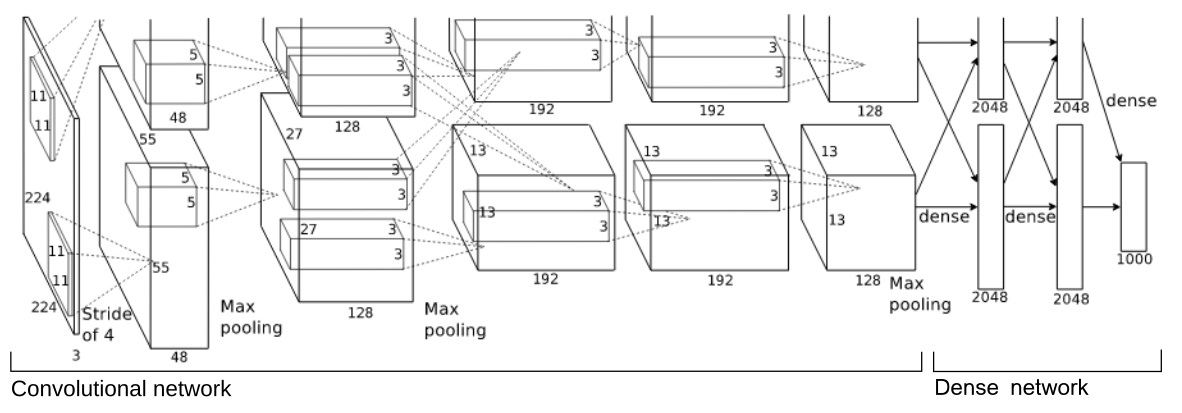
\includegraphics[width=\linewidth]{imagenet-arch}}
\end{figure}

Esta arquitectura usa en su primera parte una red convolucional preentrenada sobre un conjunto de imágenes mucho más generalista, en este caso Imagenet. Al usar una red convolucional preentrenada sobre fotografías tendrá muchas más capacidad para distinguir características de diferentes objetos, además que existen varias categorías de peces en Imagenet, por lo que sabrá diferenciar este tipo de fotografías.


\subsection{Red convolucional}

Como explicamos en el capítulo~\ref{sec:conv-net}, cuando un modelo convolucional recibe una imagen va a devolver $N$ matrices bidimensionales representando el resultado de las aplicación de los $N$ conjuntos de filtros a la imagen inicial. Al ser $N$ matrices bidimensionales también puede considerarse una matriz tridimensional.

Intuitivamente, y haciendo una simplificación, podemos pensar que cada uno de estos filtros representa un mapa de calor de la aparición en la imagen de diferentes características. Por ejemplo, ¿cúanto se parece cada parte de esta imagen a la piel de un pez?.

Hay que tener en cuenta que este modelo convolucional no ha sido entrenado con el conjunto de entrenamiento, si no con el conjunto de entrenamiento de Imagenet. Para lo único que vamos a usar esta red convolucional es para transformar estas imágenes a 

\subsection{Modelo preentrenado}

La arquitectura del artículo original \parencite{krizhevsky2012imagenet} usa capas convolucionales donde alterna filtros de $11\times11$, $5\times5$, y $3\times3$, el cual parece una buena elección para usar como modelo convolucional preentrenado. Sin embargo la aplicación de este trabajo es una competición internacional donde se usarán soluciones \textit{state of the art}. El modelo de la figura \ref{general-architecture} representa el ganador de la edición 2012 de la competición ILSVRC. Un buen punto de partida puede ser mirar los modelos ganadores de años posteriores.

El modelo principal a usar es VGG, desarrollado por el \textit{Visual Geometry Group}, de la Universidad de Oxford. Es un modelo especialmente interesante por su simplicidad, aparte de obtener una de las mejores puntuaciones en ILSVRC 2014.

\section{VGG16}

Una de las principales características de VGG es la idea de que los filtros convolucionales mayores de $3\times3$, como por ejemplo los de $5\times5$ u $11\times11$ pueden ser representados por combinaciones de filtros $3\times3$.

De las configuraciones descritas en \parencite{simonyan} hay una que sobresale por su eficiencia, llamada VGG16. Usando un total de trece capas CONV con filtros de $3\times3$, cinco capas POOL y tres capas FC (de 4096, 4096 y 1000 salidas), seguida de una función \textit{softmax} (figura \ref{vgg16-arch}), es capaz de mejorar la eficacia del modelo de Krizhevsky. El nombre de esta configuración es VGG16 ya que es la cantidad de capas CONV y FC que posee.

Estamos usando la configuración VGG16 de todas las descritas en su definición original ya que, junto con VGG19, consigue los mejores resultados.

\begin{figure}
  \caption{Arquitectura de VGG}
\label{vgg16-arch}
  \makebox[\textwidth]{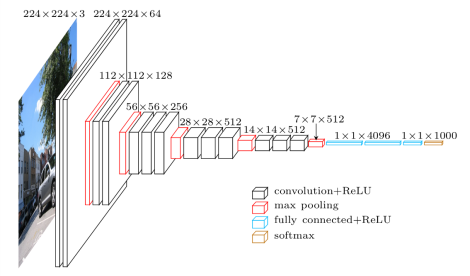
\includegraphics[width=.7\linewidth]{vgg16-arch}}
\end{figure}

\subsection{\textit{Fine-tuning}}

Si observamos la última capa del modelo VGG16, vemos que la salida tiene 1000 elementos. Tiene esta forma ya que ILSVRC consistía en clasificar una imagen entre mil categorías diferentes. Si el problema a resolver consiste en clasificar entre ocho categorías, es lógico modificar esta última capa para que tenga solo ocho salidas.

Al modificar la estructura de la última capa estamos destruyendo pesos y haciendo que muchos de los que ya existían carezcan de sentido. El hecho de que VGG tenga esta separación lógica entre la red convolucional y la red densa (las tres capas FC) hace que se pueda separar el modelo en dos modelos diferentes: uno convolucional, que no habrá cambiado con la adaptación a las ocho categorías, y otro denso, que tendrá que ser reentrenado de nuevo.

Al partir una red en dos partes diferentes hay que tener en cuenta que la segunda parte, la red densa, no recibe como entrada las imágenes, si no la salida de la red convolucional, con todas las transformaciones que esta produce. Es necesario entonces aplicar la red convolucional a todo el conjunto de datos para crear un nuevo conjunto de datos con el que reentrenar la red densa.

Esta técnica de ajustar los paŕametros de un modelo ya conocido para adaptarlo con nuevo conjunto de datos se conoce como \textit{fine-tuning}.

Usando el conjunto de datos definido en el capítulo \ref{sec:metodology}, con la separación 60\%, 20\% y 20\% para los conjuntos de entrenamiento, validación y test se ha entrenado la red densa.

Primero es necesaria la transformación del conjunto en las features producidas por la red convolucional.

\begin{python}
# Carga del modelo VGG16
from vgg16 import Vgg16
model = Vgg16()

# Diferencia entre red convolucional y densa
import utils
conv_model, dense_model = utils.split_at(model, MaxPooling2D)

# Cargamos los diferentes conjuntos de datos
train, trail_labels = get_data(path + 'train')
valid, valid_labels = get_data(path + 'valid')
test, test_labels = get_data(path + 'test')

# Convertir dataset a features mediante la red convolucional 
train_feat = conv_model.predict(train)
valid_feat = conv_model.predict(valid)
test_feat = conv_model.predict(test)
\end{python}

Este código no es completamente válido, ya que se han tomado algunas libertades para mejorar la comprensión y lectura del mismo. Define una estructura general a seguir para este problema (carga de datos, transformación, \textit{fine-tuning} y evaluación). Para una mayor comprensión el la mayor parte de las librerías usadas así como las utilidades están descritas en el Apéndice 1 (cuando lo pase a LaTex)

Una vez cargadas las librerías necesarias (Vgg16 es una clase abstracta que importa las bibliotecas necesarias de Keras), ambos modelos y transformado el dataset mediante la red convolucional se puede pasar a reentrenar la última parte de la red. Primero hay que cambiar el final de la red para conseguir que tenga ocho salidas y luego entrenar.


\begin{python}

# Cambiar el final de la red densa de 1000 outputs a 8
dense_model.pop()  # Elimina la última capa
dense_model.add(
    Dense(8, activation='softmax')  # Introducir una nueva
)

# Compilar el modelo
dense_model.compile(
    SGD(lr=0.01),
    loss='categorical_crossentropy',
    metrics=['accuracy'],  # Muestra la precision del modelo
)

# Entrenar la red
dense_model.fit(
    train_feat,
    train_labels,
    batch_size=64,  # Numero de imagenes a entrenar al mismo tiempo
    nb_epoch=7,     # Numero de iteraciones del entrenamiento
    validation_data=(valid_feat, valid_labels),
)

# Evaluar el modelo sobre el conjunto de test
dense_model.evaluate(test_feat, test_labels)
# Log loss, accurtcy
>>> [2.38985158622892523, 0.66099843993759748]
\end{python}

La puntuación total de kaggle para este conjunto de test sería $2.389$. Esto es sobre un conjunto de test muy pequeño, solo el 20\% del conjunto de entrenamiento. Como se ya ha dicho anteriormente habría que mandar las predicciones del conjunto de test final a kaggle para verificar la puntuación del modelo, pero por problemas de restricciones esta es la forma de medir los modelos generados.

El segundo número que devuelve la función $evaluate$ es la precisón ($accuracy$) del modelo. Al ser el modelo un modelo de clasificación, el mandar $"accuracy"$ como parámetro a la hora de compilar el modelo hace que eliga como métrica la precisión por categorías. Esto va a devolver el porcentaje de veces que la clase con la probabilidad máxima se corresponde con la clase etiquetada en el dataset. En este caso el modelo ha adivinado correctamente el 66\% de las imágenes, un número muy aceptable teniendo en cuenta que solo se ha tocado la capa final de un modelo ajeno.

\section{Modelo personalizado}

La idea original que se comentaba al principio consistía en separar el problema en el modelo convolucional y el modelo de clasificación. Es en el segundo donde se puede conseguir toda la flexibilidad. 

El modelo original de VGG usa dos capas $densas$ de 4096 neuronas para clasificar entre mil clases diferentes. Ya que este problema tiene solo ocho clases diferentes probablemente no sea necesario usar capas tan grandes, por lo que se procede a probar la misma estructura original pero con capas cuatro veces más pequeñas que las originales.

La estructura, por lo tanto, quedaría de la misma manera pero usando dos capas densas de 512 neuronas cada una y una capa densa final de 8. Para no tener que estar modificando el modelo original cada vez que haga falta es mucho más sencillo crear un modelo nuevo con $Keras$ y añadir todas las capas necesarias.

\begin{python}
def build_dense_layers():
    return [
        Flatten(),
        Dense(512, activation='relu'),
        Dense(512, activation='relu'),
        Dense(8, activation='softmax')
    ]

dense_model = keras.models.Sequential(build_class_layers())
\end{python}

Un paso importante a la hora de construir el modelo personalizado es tener en cuenta que las salidas de las redes convolucionales poseen tres dimensiones ($ancho \times alto \times filtros$), mientras que la redes neuronales densas poseen solo una dimensión. Es necesario convertir la salida de estas capas a una entrada permitida. Keras ya ofrece esta posibilidad usando una capa abstracta llamada Flatten.

\begin{python}
# Entrenar la red
dense_model.compile(...)
dense_model.fit(...)
# Evaluar el modelo sobre el conjunto de test
dense_model.evaluate(test_feat, test_labels)
>>> [1.27721316430079874, 0.69567862714508579]
\end{python}

Los resultados obtenidos son ligeramente mejores que los anteriores, sin embargo no es aquí donde está toda la mejora. El entrenamiento de este modelo ha sido un 80\% más rápido que el anterior (19.5 segundos el primero, 3.9 segundos el último). Esto no solo ha permitido entrenar la red durante más tiempo, si no que en el futuro hará posible entrenar sobre mayores cantidades de datos sin sacrificar velocidad.

\subsection{Mejorar el modelo}

La salida de Keras al entrenar el modelo ofrece información de lo que está sucediendo. Este es un ejemplo de la salida del entrenamiento del modelo anterior.

\begin{python}
Epoch 5/7
loss: 1.406 - acc: 0.621 - val_loss: 2.0197 - val_acc: 1.861
Epoch 6/7
loss: 0.992 - acc: 0.674 - val_loss: 1.4356 - val_acc: 1.001
Epoch 7/7
loss: 0.872 - acc: 0.761 - val_loss: 1.2772 - val_acc: 0.695
\end{python}

Los valores mostrados indican los resultados de la evaluación del modelo sobre el conjunto de entrenamiento y el de validación, respectivamente. Esto es mostrado para cada uno de los pasos. Se puede observar que el modelo funciona mucho mejor en el conjunto de entrenamiento que en el de evaluación.

Cuando un modelo tiene demasiados parámetros y ha sido entrenado durante demasiado tiempo aprende a clasificar los ejemplos con los que entrena, usando información específica de cada uno de ellos en vez de generalizar. Esto se conoce como \textbf{sobreajuste} (\textit{overfitting}).

Los datos del modelo anterior indican que puede existir un sobreajuste, por lo que se va a intentar tomar medidas para arreglarlo.

\subsection{Dropout}

Una de las características de VGG y otras redes convolucionales es el uso de \textit{Dropout} para reducir el sobreajuste de los modelos entrenados. El \textit{Dropout} consiste en una capa que se aplica después de las capas de activación. Esta capa convierte activaciones aleatorias a 0, eliminando la información transportada.

En un principio parecería que esto perjudica al modelo, pero al eliminar algunos de los pesos el modelo evita centrarse en características individuales de cada ejemplo de clasificación, obligándolo a generalizar más rápido \parencite{krizhevsky2012imagenet}.

Un pequeño experimento en un modelo más avanzado (VGG con \textit{batch normalization} y aumento de datos) permite ver  como afecta el \textit{dropout} a la puntuación final. En la figura \ref{dropout} se puede observar que la mejor puntuación se alcanza eliminando el 45\% de las activaciones, consiguiendo una mejora de un 25\% sobre el modelo que usa todas las activaciones.

\begin{figure}
    \caption{Evolución de la puntuación de un modelo usando \textit{dropout}}
\label{dropout}
  \makebox[\textwidth]{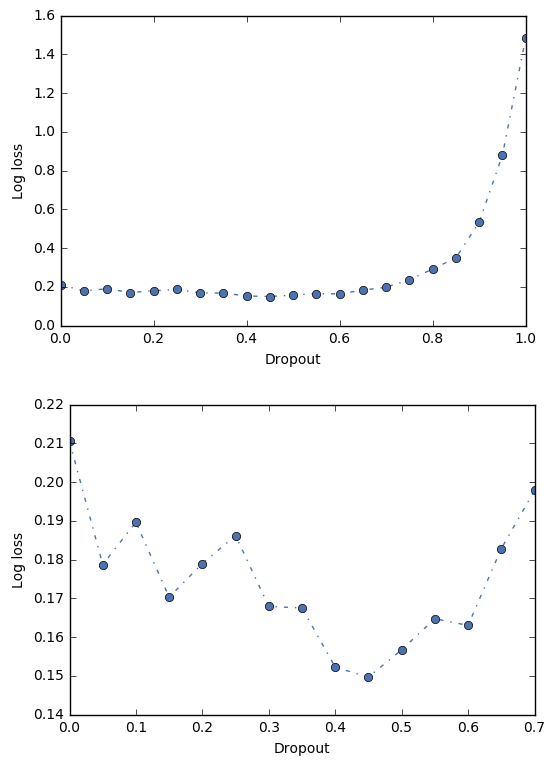
\includegraphics[width=0.7\linewidth]{dropout}}
\end{figure}


También se ve que el modelo empieza a perder eficacia a partir del 70\% de \textit{dropout}, empeorando el modelo original. Esto significa que el modelo es capaz de generalizar con información útil incluso cuando solo posee el 30\% de las activaciones.

Por otra parte también es importante pensar dónde se pierden las activaciones. Por un lado, perder demasiadas activaciones en la entrada sería el equivalente a trabajar sin esos ejemplos. Por otro, perderlos en la salida sería aumentar demasiado el error al clasificar. La idea aplicada aquí es distribuir el \textit{dropout} disminuyéndolo en la entrada y la salida y haciendo que tenga su punto máximo en el centro de la red.

La definición de la red anterior quedaría de la siguiente manera:

\begin{python}
def build_dense_layers(p):
    return [
        Flatten(),
        Dropout(p/4)
        Dense(512, activation='relu'),
        Dropout(p)
        Dense(512, activation='relu'),
        Dropout(p/2)
        Dense(8, activation='softmax')
    ]
dense_model = keras.models.Sequential(build_class_layers(0.45))
\end{python}

Los resultados obtenidos con esta configuracion no mejoran mejoran los resultados de la red anterior, pero como se ve en la figura \ref{dropout} sí que lo hará a posteriori, cuando se le apliquen otro tipo de mejoras al modelo.

\subsection{Batch normalization}

\subsection{Data augmentation}

En muchos algoritmos de 
\subsection{Fully convolutional network}

